\chapter{Аналоговая модуляция}

\section{Цель работы}
Изучение амплитудной модуляции/демодуляции сигнала.

\section{Ход работы}

\subsection{Теоретическая часть}
* $S(t)$ — информационный сигнал, $|S(t)|<1$,

* $U_c(t)$ — несущее колебание.

Тогда амплитудно-модулированный сигнал $U_\text{am}(t)$ может быть записан следующим образом:
$$U_\text{am}(t)=U_c(t)[1+mS(t)] (1)$$
Здесь $m$ — некоторая константа, называемая коэффициентом модуляции. Формула описывает несущий сигнал $U_c(t)$, модулированный по амплитуде сигналом $S(t)$ с коэффициентом модуляции $m$.

\subsection{Код Matlab}
\begin{lstlisting}
close all;
clear all;

x = 0:0.1:8*3.14;
f0 = 0.1;

% Исходный сигнал
y = sin(2*pi*f0*x);
figure
plot(x(1:250),y(1:250))
grid

% Спектр исходного сигнала
spectrum = fft(y, 512);
norm_spectrum = spectrum.*conj(spectrum)/512;
f = 100*(0:255)/512;
figure
plot(f, norm_spectrum(1:256))
axis([0 max(f) 0 70])
grid

% Амплитудная модуляция
Fc = 10*f0;
Fs = 100*f0;
U = ammod(y, Fc, Fs, 0, 1);
figure 
plot(x(1:250), U(1:250))
grid

 % Спектр модулированного сигнала
 u_spectrum = fft(U, 512);
 norm_u_spectrum = u_spectrum.*conj(u_spectrum)/512;
 figure
 plot(f, norm_u_spectrum(1:256))
 axis([0 max(f) 0 70])
 grid

% Амплитудная модуляция с подавлением несущей
Fc = 10*f0;
Fs = 100*f0;
U = ammod(y, Fc, Fs);
figure 
plot(x(1:250), U(1:250))
grid

% Спектр модулированного сигнала
u_spectrum = fft(U, 512);
norm_u_spectrum = u_spectrum.*conj(u_spectrum)/512;
figure
plot(f, norm_u_spectrum(1:256))
axis([0 max(f) 0 70])
grid

% Однополосная модуляция
Fc = 10*f0;
Fs = 100*f0;
U = ssbmod(y, Fc, Fs, [], 'upper');
figure 
plot(x(1:250), U(1:250))
grid

% Спектр модулированного сигнала
u_spectrum = fft(U, 512);
norm_u_spectrum = u_spectrum.*conj(u_spectrum)/512;
figure
plot(f, norm_u_spectrum(1:256))
axis([0 max(f) 0 70])
grid

%Синхронное детектирование
[b, a] = butter(10, Fc*2/Fs);
z = ssbdemod(U, Fc, Fs, 0, b, a);
figure
plot(x(1:250), z(1:250))
grid

% Спектр демодулированного сигнала
du_spectrum = fft(U, 512);
norm_du_spectrum = du_spectrum.*conj(du_spectrum)/512;
figure
plot(f, norm_du_spectrum(1:256))
axis([0 max(f) 0 70])
grid

% Рассчет КПД модуляции 
M = 0.5;
n = M^2/(M^2+2)

\end{lstlisting}

\begin{figure}[H]
   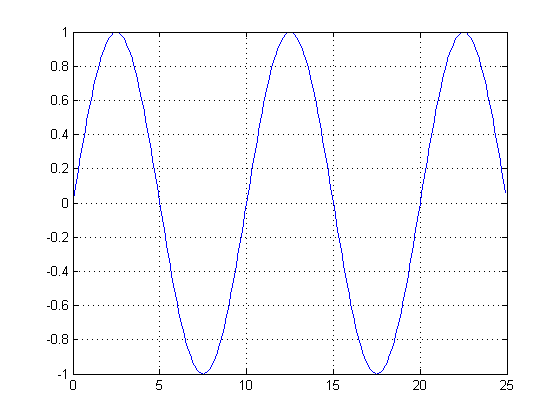
\includegraphics[scale=0.7]{lab7/src_signal.png}
   \caption{Исходный сигнал}
\end{figure}

\begin{figure}[H]
   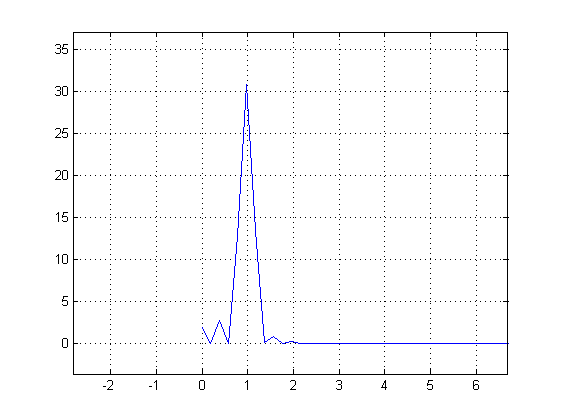
\includegraphics[scale=0.7]{lab7/src_signal_spectro.png}
   \caption{Спектр исходного сигнала}
\end{figure}

\begin{figure}[H]
   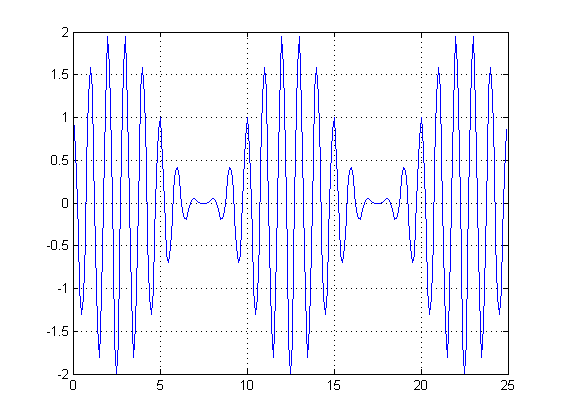
\includegraphics[scale=0.7]{lab7/AM.png}
   \caption{Амплитудная модуляция}
\end{figure}

\begin{figure}[H]
   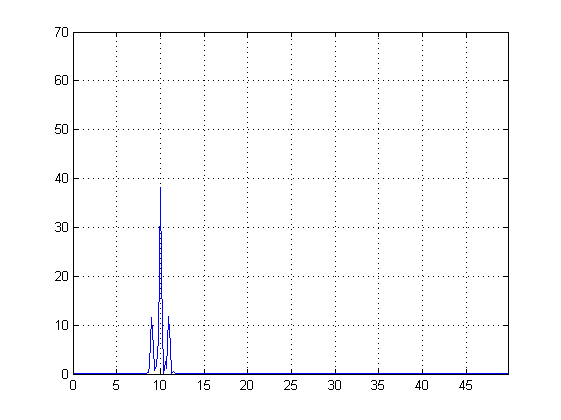
\includegraphics[scale=0.7]{lab7/AM_spectro.png}
   \caption{Спектр модулированного сигнала}
\end{figure}

\begin{figure}[H]
   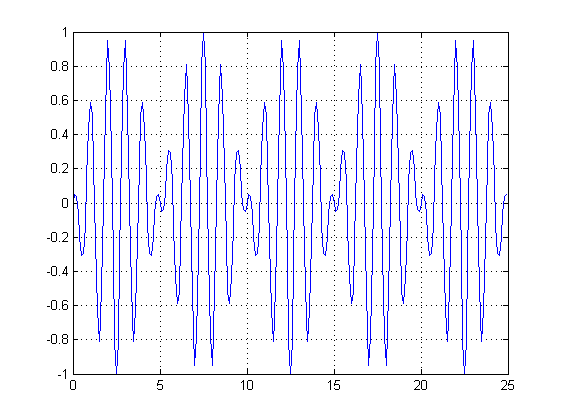
\includegraphics[scale=0.7]{lab7/ammod.png}
   \caption{Амплитудная модуляция с подавлением несущей}
\end{figure}

\begin{figure}[H]
   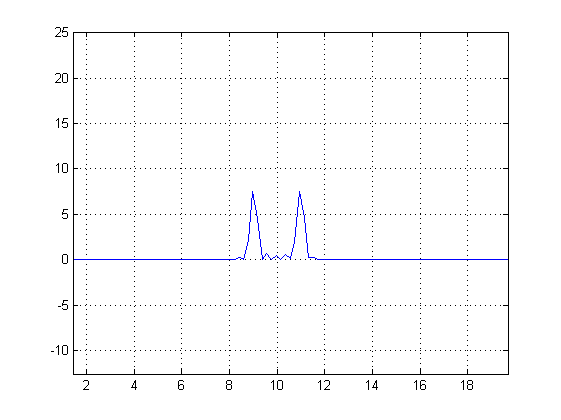
\includegraphics[scale=0.7]{lab7/ammod_spectro.png}
   \caption{Спектр модулированного сигнала}
\end{figure}

\begin{figure}[H]
   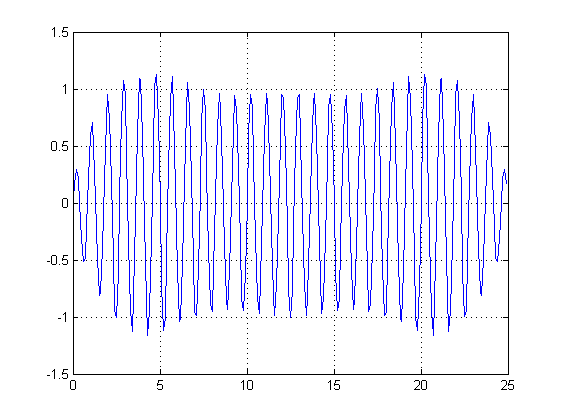
\includegraphics[scale=0.7]{lab7/ssbmod.png}
   \caption{Однополосная модуляция}
\end{figure}

\begin{figure}[H]
   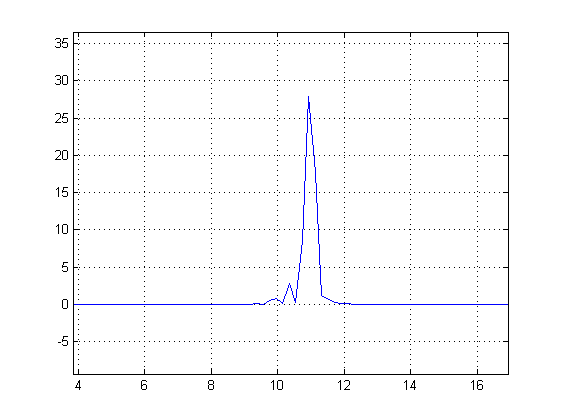
\includegraphics[scale=0.7]{lab7/ssbmod_spectro.png}
   \caption{Спектр модулированного сигнала}
\end{figure}

\begin{figure}[H]
   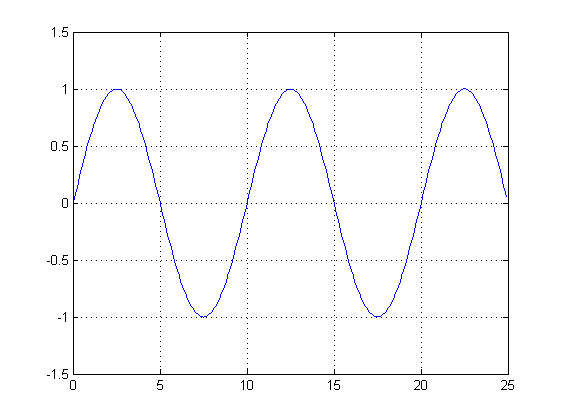
\includegraphics[scale=0.7]{lab7/ssbdemod.png}
   \caption{Синхронное детектирование}
\end{figure}

\begin{figure}[H]
   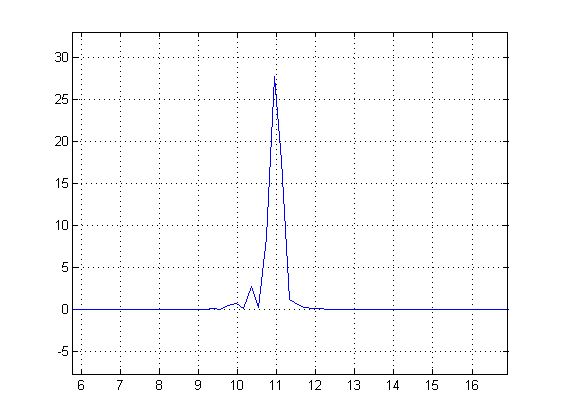
\includegraphics[scale=0.7]{lab7/ssbdemod_spectro.png}
   \caption{Спектр модулированного сигнала}
\end{figure}


\subsection{Simulink}

\begin{figure}[H]
   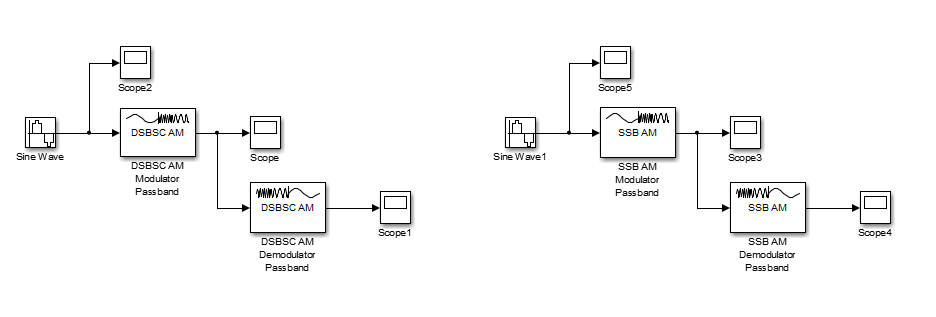
\includegraphics[scale=0.5]{lab7/sim_lab7.png}
   \caption{Схема модели}
\end{figure}

%\begin{figure}[H]
%   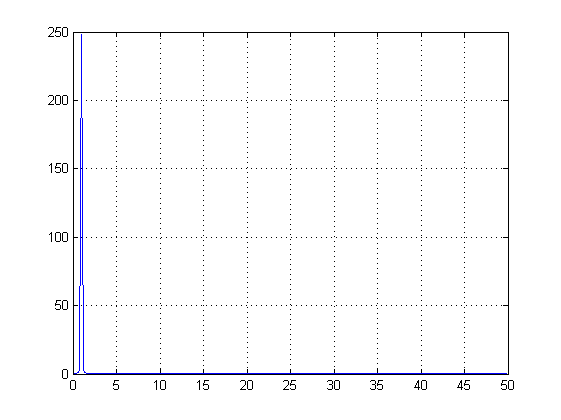
\includegraphics[scale=0.7]{lab7/11.png}
%   \caption{Исходный сигнал}
%\end{figure}

\begin{figure}[H]
   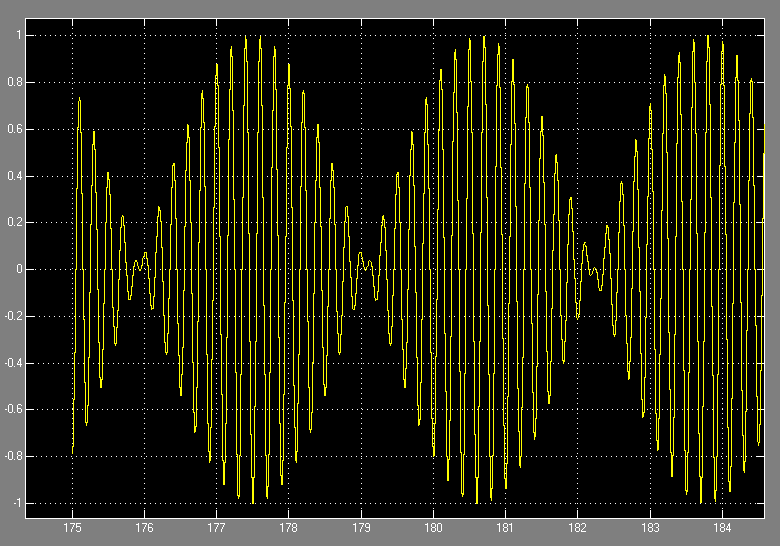
\includegraphics[scale=0.5]{lab7/Scope.png}
   \caption{Модулированный сигнал}
\end{figure}
\begin{figure}[H]
   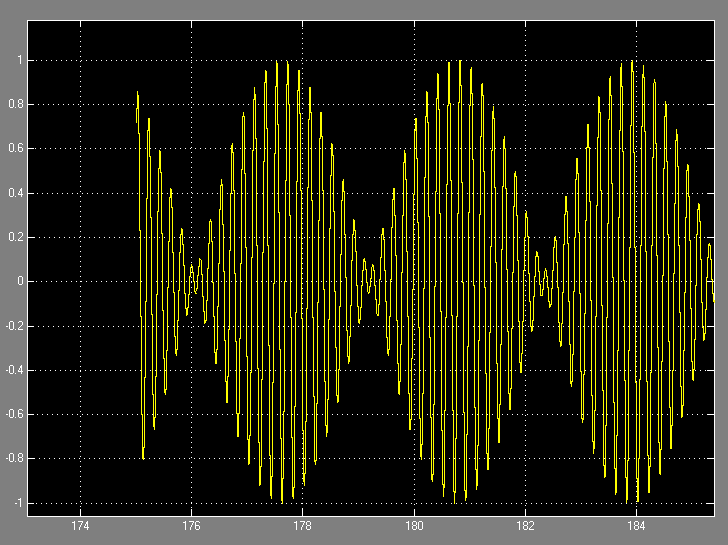
\includegraphics[scale=0.5]{lab7/Scope3.png}
   \caption{Демодулированный сигнал}
\end{figure}



\section{Вывод}
В настоящее время амплитудная модуляция применяется в основном только для радиовещания на сравнительно низких частотах (не выше коротких волн) и для передачи изображения в телевизионном вещании. Это обусловлено низким КПД использования энергии модулированных сигналов. АМ - сигнал представляет собой произведение информационной огибающей U(t)
и гармонического колебания ее заполнения с более высокими частотами.
Значение М должно находиться в пределах от 0 до 1 для всех гармоник модулирующего сигнала. При значении M < 1 форма огибающей несущего колебания полностью повторяет форму модулирующего сигнала s(t). Малую
глубину модуляции для основных гармоник модулирующего сигнала(M <<1) применять нецелесообразно, т.к. при этом мощность передаваемого информационного сигнала будет много меньше мощности несущего колебания,
и мощность передатчика используется неэкономично. Для однотональной
модуляции начальная фаза модулирующего колебания для верхней боковой частоты складывается с начальной фазой несущей, для нижней - вычитаются из фазы несущей. Физическая ширина спектра модулированного
сигнала в два раза больше ширины спектра сигнала модуляции, так как
модулирующее колебание перемещается в область частоты $\omega_0$ и расщепляется на два колебания, симметричные относительно частоты $\omega_0$, что будет видно в спектре.
$$ u(t) = U_m cos(\omega_0 t) + (U_m * M/2)cos[(\omega_0 + \Omega)t] + (U_m * M/2)cos[(\omega_0 - \Omega)t] $$
При балансной модуляции производится перемножение двух сигналов - модулирующего и несущего, при котором происходит подавление несущего колебания, соответственно, КПД модуляции становится равным 100\%.
